
\section{Introduction}%
\label{sec:introduction}

La PMF étant un modèle d'apprentissage statistique, le regroupement des espèces chimiques
en différent facteurs est sensible à la méthodologie employée et au jeu de variable
utilisé.
Depuis plusieurs années, les travaux du groupes essaient d'évaluer la pertinence de
l'ajout de nouveaux traceurs dans les études PMF, afin de mieux prendre en compte
certaines émissions anthropiques ou biogéniques mais également afin de mieux estimer la
contribution des aérosols secondaires, qu'ils soient organiques ou inorganique.
En plus d'identifier plus précisément ces sources, \cite{emamiEffect2017} ont montré que
l'ajout d'espèce traceuse permet une diminution de l'ambiguité rotationelle pour
l'ensemble des facteurs identifiés. La recherche de nouvelles espèces traceuses est donc
nécessaire pour identifier de nouvelles sources, mais également diminuer l'incertitudes
sur celles déjà bien établies.

À ce titre, le site de Grenoble les Frènes a permis le prélèvement et analyse de composés
organiques (HULIS, hopanes, oxy- et nitro-HAP ainsi que oxy- et nitro-HAPs) permettant de mettre en
évidence la saisonalité de ces composés, tracant différent processus : émissions lié à la
combustion en hiver pour les oxy- et nitro-HAP ainsi que leur transport longue distance
alors que les oxy- et nitro-HAPs semblent quand à eux être d'avantage liés aux processus
d'oxydation secondaires du fait de leur corrélation avec
l'oxalate~\textcite{tomazSources2017a}.
Lors d'études PMF avec ces traceurs \autocite{srivastavaSpeciation2018a}, il ressort bien
qu'une part de ces espèces est associés à la combustion de biomasse mais ont aussi permis
la mise en évidence d'un facteur anthropique secondaire présentant un signal assez
atypique car très ponctuel. Aussi, les processus d'oxydation secondaires de la matière
organique est mieux déterminé et quantifiée, ce qui a permis d'isolé un facteur biogenique
secondaire présentant de forte concentration en été. Quand au trafic routier, la grande
majorité des hopanes se retrouvent dans ce facteurs, alors certains autres composés pour
lesquels des fortes concentrations étaient attendues sont en définitive peu présents dans
ce facteur (notamment pour le 1-nitropyrène \textcite{ringuetDiurnal2012}).

Cependant, certains de ces composés présentent des faibles performances statistiques (i.e.
concentration observées vs reconstruites) et soulèvent différentes intérogations : faut-il
utiliser toutes ces espèces en même temps ? Faut-il aggréger certaines familles de
composés mono-source ? Est-ce que la résolution de 24h est suffisante ?  etc. D'autres
travaux en ce sens ont eu lieu sur le site expérimental de Lens, en sommant par exemple
certaines espèces (hopanes, alcanes, HAP) afin de réduire le nombre d'espèces utilisées
dans la PMF, mais aucun standard n'existe à ce jours et peu d'études rapportent
l'utilisation de ces traceurs dans les PMF.
Aussi, la variabilité spatiale de ces profils semblent être importante. Dans des travaux en
cours de la thèse de Valéria Mardonnez à La Paz, Bolivie, la dynamique de ces composés
dans les PMF permettraient d'identifier jusqu'à 3 facteurs reliés au trafic routier : selon
la source de combustion (diesel ou essence) et émission hors-combustion.

Mais d'autres voies d'ajout de traceurs sont également à l'étude, cherchant à coupler les
mesure sur filtre à d'autres mesures concommitante \parencite{srivastavaSpeciation2019}.
Récemment, la thèse de Florie Chevrier \autocite{chevrierChauffage2016} dans le cadre du
programme DECOMBIO a permis la combinaison de mesure issues de chimie sur filtre,
d'aethalometre (séparant ainsi le BC en combustion de biomasse et combustion fossile) et
mesure de \ce{^{14}C}.

Ainsi, la méthodologie d'utilisation du modèle PMF est encore actuellement en évolution,
et ce chapitre discutera des différentes avancées ou pistes que ma thèse a exploré ces
dernières années.

\section{Validation externe des solutions PMF}%
\label{sec:confrontation_des_solutions_pmf}

Comme discuter précédemment, un modèle doit être évaluer par des mesures externes. Or, il
est compliquer voir impossible de « mesurer » la concentration des sources de PM (c'est
justement le travail demandé à la PMF). On ne peut donc faire que des confrontations
indirectes, à travers d'autres types de mesure ou modèle, chimique ou géophysique, afin
d'estimer la fiabilité d'une solution PMF.

\subsection{Confrontation aux mesures de radiocarbone \ce{^{14}C}}%
\label{sub:14c}

Sur les sites de la vallée de l'Arve dans le cadre du programme DECOMBIO, en plus des mesures
traditionelles sur filtre, \textcite{bonvalotEstimating2016} ont également estimé par
traçage isotopique au radiocarbone \ce{^{14}C} l'origine fossile ou récente du carbone.
Les études PMF sur le site de Passy et Chamonix de \textcite{chevrierChauffage2016},
illustrées figure~\ref{fig:chapter03/radiocarbon_chevrier_winter} ont
montrées une très bonne concordance entre la quantité de carbone provenant de source
fossile estimée par radiocarbone et les facteurs PMF traçant des sources de combustion de
carbone fossil. Réciproquement, le carbone récent est en très bon accord entre les mesures
radiocarbone et PMF.

Cette confrontation à des mesures externes à la PMF conduisant à des résultats concordant
accentue fortement la confiance que l'on peut avoir dans les résultats et la
quantification de la contribution des sources issues de ces analyses.

\begin{figure}[ht]
    \centering
    \includegraphics[width=1.0\linewidth]{chapter03/radiocarbon_chevrier_winter.png}
    \caption{Contributions relatives au carbone total en moyennes hivernales des sources
        de \PMdix identifiées lors de la thèse de \textcite{chevrierChauffage2016} par les
        différentes approches PMF et contributions des parts fossile et non-fossile
        obtenues par l’analyse du radiocarbone de \textcite{bonvalotEstimating2016}.
    Source: \textcite[figure 75]{chevrierChauffage2016}}%
    \label{fig:chapter03/radiocarbon_chevrier_winter}
\end{figure}

\subsection{Confrontation mesure sur site récepteur et origine géographique}%
\label{sub:confrontation_mesure_sur_site_recepteur_et_origine_geographique}

Les facteurs PMF étant déterminer au niveau du site recepteur mais n'étant pas
nécessairement émis à cet endroit spécifique, il est également possible d'estimer leur
provenance géographique et leur vraisemblance. Nous verrons d'abord le cas simple de la
rose des polluants, avant d'expliciter plus en avant la méthode PSCF.


\subsubsection{Cas simple : la rose des polluants}%
\label{ssub:cas_simple_la_rose_des_polluants}

L'un des moyens les plus simples pour cela est de coupler des mesures de direction et
vitesse de vent et d'établir une rose des polluants. J'ai pu utiliser ce procédé à des
fins exploratoires lors de ma thèse, ce qui m'a conduit à contribuer au développement de
\href{https://github.com/python-windrose/windrose/}{windrose}~\autocite{scls19frPythonwindrose2019}.
Cependant, cette méthode n'est utile que pour la détermination de source proche du site
récepteur car dès lors que l'on s'en éloigne, l'orientation et vitesse des vents varient
et l'hypothèse de déplacement uniforme de la masse d'air est invalidée.  Or, il est
courant que les aérosols proviennent de sources non locales, limitant l'utilisabilité de
cette méthode.


\subsubsection{Prendre en compte l'histoire de la masse d'air : PSCF}%
\label{sub:prendre_en_compte_l_histoire_de_la_masse_d_air_PSCF}

Pour s'affranchir de la limitation des rose des vents, il est possible d'utiliser les
rétrotrajectoires complètes des masses d'air pour remonter aux sources géographiques
potentielles, mais également de coupler ces trajectoires à des informations
physico-chimiques comme la concentration en polluants observés sur le site récepteur, la
présence de pluie sédimentant les aérosols par dépôt humide ou encore la hauteur de la
masse d'air.

L'une des méthodes les plus largement utilisée dans la littérature est la \textit{Potential
source contribution function} (PSCF), permettant de combiner des ensembles de trajectoires à
des modèles récepteurs. Le principe consiste à calculer les rétrotrajectoires d'un site
récepteur donné et d'associer à chacune d'elle la concentration du polluant ou de la
source considéré le jour de son passage au niveau du site récepteur. En discrétisant les
trajectoires en 1 point toutes les X minutes ou heures et en appliquant une grille
régionale, il est alors possible de dénombrer combien de rétrotrajectoires sont passés par
chacune des grilles.  Le ratio du nombre de trajectoire associée à une forte concentration
aux coordonnées $i$, $j$, noté $m_{ij}$, par le nombre total de trajectoire étant passé
par ces coordonnés notées $n_{ij}$, nous donne une probabilité de provenance géographique
de ce composé ou source pour les coordonnées $i$, $j$, noté $PSCF_{ij}$ :
\begin{align}
    \label{eq:PSCF}
    PSCF_{ij} &= \frac{m_{ij}}{n_{ij}}.
\end{align}

Des améliorations ont été apportées à cette méthode afin de prendre en compte les cellules
ayant un faible pourcentage de passage de rétrotrajectoires, augmentant artificiellement
le ratio $\frac{M}{N}$. Une manière de contrebalancer ce biais et d'ajouter une fonction
poids, dépendant de la fréquence de passage des rétrotrajectoires sur chacune des
cellules. Dans la figure~\ref{fig:chapter02/PSCF_method}, illustrant la PSCF, on voit que
la cellule où 2 rétrotrajectoires sont passés se voit attribuer la même probabilité que
celles avoisinantes, où seule une rétrotrajectoire a résidé. Or, il serait plus pertinent
d'avoir une probabilité plus forte pour cette cellule, indiquant que chaque
rétrotrajectoire ayant résidé à ces coordonnées est riche du composé suivit.  Différentes
fonctions poids existent, le plus souvent présentant différents seuils en fonction du
nombre de rétrotrajectoires par cellule~\autocite{bressiSources2014,petitSources2019}.

Aussi, pour avoir une représentativité statistique suffisante des sources potentielles, il
est nécessaire de calculer un grand nombre de rétrotajectoire, correspondant à chacun des
jours de prélèvement sur le site récepteur.


\begin{figure}[ht]
    \centering
    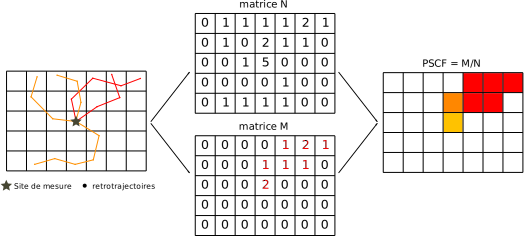
\includegraphics[width=0.9\linewidth]{chapter03/PSCF_method.pdf}
    \caption{Illustration de la méthode PSCF : les rétrotrajectoires depuis le site de
        mesure sont calculées, celles associées à une concentration seuil sont
        représentées en rouge, les autres en orange. Les matrices N et M s'obtiennent par
        simple décompte du nombre de rétrotrajectoires passés dans chaque cellule de
        taille prédéfinies, puis le ratio nous donne une estimation de l'origine
    géographique, représentée ici terme d'intensité de rouge.}%
    \label{fig:chapter02/PSCF_method}
\end{figure}

\subsubsection{Automatisation et simplification : pyPSCF}%
\label{ssub:automatisation_et_simplification_pypscf}

Ces étapes fastidieuses de calcul des rétrotrajectoires et de PSCF ont été automatisés
dans un paquet python, pyPSCF\footnote{Dépot git pyPSCF:
\url{https://gricad-gitlab.univ-grenoble-alpes.fr/webersa/pyPSCF}}, permettant le
traitement d'un grand nombre de rétrotrajectoire en utilisant le modèle lagrangian
HYSPLIT et calculant de manière facilité une PSCF en un site donné, en variant notamment
les différents paramètres succeptibles d'influencer le modèle.

Également, et de manière similaire à ZeFir de \textcite{petitUserfriendly2017}, pyPSCF
propose une interface utilisateur permettant une interaction facilité.

\subsubsection{Application de la PSCF}%
\label{ssub:application_de_la_pscf}

\paragraph{Importance et origine géographique du MSA ? (Golly et al. 2019)}%
\label{par:origine_terrestre_ou_marine_du_msa_}

Comme expliqué précemment, une part importante des aérosols provient de sources
secondaires, c'est-à-dire du vieillissement et des réactions dans l'atmosphère. Une part
importante de ces aérosols secondaires sont d'origines organiques. Les travaux
de~\textcite{gollyOrganic2019}, auxquels j'ai pris part, s'attachent notamment à la
quantification de cette matière organique secondaire sur 5 sites ruraux en France
pendant l'année 2013, par la mesure de deux espèces issues de processus secondaires : le
MSA et l'oxalate.  Nous avons pu montrer que le MSA, considéré comme provenant de
l'oxydation du DMS, peut contribuer jusqu'à 10 à 20\% de l'OC en période chaude,
indiquant une forte proportion d'aérosols organiques secondaires durant l'été. Mais
surtout, le MSA est considéré comme provenant des émissions de DMS du phytoplanction
marin, au point qu'il est proposé comme méthode de séparation entre le sulfate d'origine
marine et ses autres provenances.

En conduisant une analyses PSCF sur les 25\% des jours les plus fortement chargés en MSA,
nous avons pu confirmer l'importance marine de ce composé, mais également montrer qu'une
part non négligeable semble provenir d'environnement terrigène (voir
figure~\ref{fig:chapter03/golly_PSCF_MSA}), confortant les études suggérants des
processus d'émissions du MSA par des sources biologiques
terrestres~\autocite{bozzettiArgon2017}, pouvant provenir des forêts ou des
sols~\autocite{jardineDimethyl2015,miyazakiSeasonal2012}.

L'une des implications directes de ces travaux résulte en l'ajout systématique du MSA
comme variable d'entrée des études PMF, quelque soit leur localisation. En effet, le
signal du MSA est clairement distinct des autres espèces chimiques mesurées et représente
également une part important de la matière organique. Cette espèce est donc a minima
traceuse de processus secondaires présents sur l'ensemble de l'europe occidentale.

\begin{figure}[ht!]
    \centering
    \includegraphics[width=0.9\linewidth]{chapter03/golly_PSCF_MSA.png}
    \caption{Probabilité de l'origine géographique du MSA, issue de l'article
        de~\textcite{gollyOrganic2019}. Bien que l'on retrouve l'origine marine du MSA,
        les sites de Dieulefit, OPE ou Peyrusse-Vieille indiquent également une forte
        probabilité d'origine terrestre de ce composé.}%
    \label{fig:chapter03/golly_PSCF_MSA}
\end{figure}

\paragraph{Confrontation PSCF -- PMF}%
\label{par:confrontation_pscf_pmf}

Une autre utilisation de la PSCF consiste à croiser les informations issues de la PSCF et
des PMF.
En effet, il n'existe pas de moyen simple de valider le sens géochimique d'une solution
PMF autrement que l'expertise et les connaissances de l'utilisateur.

Pour estimer la fiabilité de la solution obtenue, il est possible de conduire une
étude PSCF sur les différents facteurs identifiés. On s'attend à ce que le
facteur \textit{sel de mer} provienne géographiquement d'un océan ou d'une mer par
exemple.

Un exemple d'utilisation de ce procédé est expliqué et illustré dans la section dédié aux
PMF et isotopie, section~\ref{sub:isotopie}.



\section{Incertitudes associées aux PMF}%
\label{sub:incertitudes_associées}

Le modèle PMF est maintenant relativement courrament utilisés dans le domaine de la
qualité de l'air. Seulement, peu d'étude rapportent en même temps que leur solution
finale, les incertitudes associées. Or, le solveur ME-2 permet l'estimation de ces
incertitudes à travers les méthodes de bootstrap et de displacment (voir
section~\ref{par:incertitudes}).

Seulement, ces incertitudes ne sont rapportées par l'EPAPMF5.0 que pour les concentrations
des espèces chimiques des différents facteurs et non pour leurs contributions temporelles.
Notamment, leur de l'estimation de la variabilité via bootstrap, les différents facteurs
sont attribués aux facteurs de références d'après leur corrélation temporelle (par défaut
$r > 0.6$), mais seul les profils chimiques sont rendu à l'utilisateur par la suite.
Une solution serait de manuellement explorer 100 solutions PMF, avec ou sans tirage
aléatoire des échantillons, pour estimer respectivement la variabilité provennant du modèle
statistique ou de la représentativité du jeu de donnée. Malheureusement, cette
répétabilité est beaucoup trop fastidieuse à faire à la main et ne peut pas s'automatiser à
partir de l'EPAPMF5.0. Or, il s'agit de l'implémentation du ME-2 le plus largement
utilisée. C'est pourtant une besoin important lors de la transférabilité de nos recherches
vers l'opérationnel, avec des questions très pratique cherchant l'incertitude
sur la contribution de telle source pour tel jours de pic de pollution en particulier.

Une ``astuce'' consiste alors a réestimer la variabilité des contributions temporelles
$X_{err}$ à partir de la variabilité de la composition chimique des profiles, i.e. en gardant
$G$ fixe (celle de référence, $G_{ref}$) mais en utilisant les profiles $F_{err}$ issue
des bootstraps et ambiguité rotationelle :
\begin{align}
    \label{eq:hack_unc}
    X_{err} &= G_{ref} \times F_{err}.
\end{align}

Même si en théorie pour la méthode du bootstrap à la fois $G$ et $F$ doivent
évoluer en même temps, cela donne une première estimation de la gamme d'incertitude pour
chaque espèce et chaques jours d'observation.

Cette visualisation, présentée à titre d'exemple pour la PMF de Vif
figure~\ref{fig:chapter03/vif_nitraterich_all} permet de rapidement se rendre compte du
type d'incertitude prépondérant pour chacune des espèces (représentativité de
l'échantillonage et ambiguité rotationelle) mais également de la gamme de valeur possible
pour chaque jours étant donnée les incertitudes estimées.

\begin{figure}[ht]
    \centering
    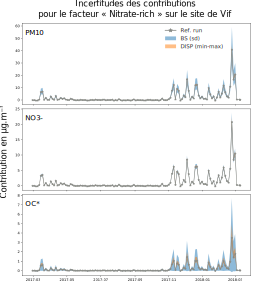
\includegraphics[width=0.8\linewidth]{chapter03/vif_nitraterich_all.pdf}
    \caption{Incertitudes temporelles des concentrations de \PMdix, \NOt et OC* dans le
    facteur Nitrate-rich de Vif estimée par boostrap (écart type de 100 bootstrap en bleu)
et displacment (min et max en orange). La solution de référence est représenté par les
trais et étoiles grisent.}%
    \label{fig:chapter03/vif_nitraterich_all}
\end{figure}


\section{Comparabilité des solutions}%
\label{sub:comparabilité_des_solutions}

Une problématique récurrente lors de l'utilisation des PMF est de se demander si les
profils que l'on obtient seraient nommés de la même façons par d'autres utilisateurs, et
si oui, comment peut-on évaluer la proximité géochimique de facteurs identiquement nommés
en différents endroits (spatiallement ou temporellement).

Les travaux de \cite{belisNew2015a} suggèrent l'utilisation conjointe de 2
métriques permettant d'estimer la distance géochimique entre 2 profiles de facteurs.

\subsection{Méthodologie}%
\label{sub:méthodologie}

\paragraph{Distance de Pearson}%
\label{par:distance_de_pearson}

La distance de Pearson (\textit{Pearson distance} PD) estime la proximité entre 2 série de
donnée en utilisant leur corrélation de Pearson, soit :
\begin{align}
    \label{eq:PD}
    PD &= 1 - r^2
\end{align}
avec $r$ la correlation entre les 2 séries de données. Pour les profiles chimiqes des
facteurs, il s'agit de la concentration relative des espèces chimiques les constituants
(i.e. pourcentage massique de chacune des espèces).

Seulement, cette distance est très sensible aux extrêmes du fait de sa dépendance au
coefficient de correlation. Ainsi, si seul l'OC est similaire pour les 2 profiles mais la
totalité des métaux présentent des concentrations très différentes, alors le PD pourra
être acceptable car l'OC présente des concentrations relative bien supérieure à celles
des métaux (voir figure~\ref{fig:chapter03/PD_belis2015a}).
De plus, la distance de Pearson ne teste que l'hypothèse de relation linéaire entre les
deux profiles, et non leur égalité stricte.

\begin{figure}[ht]
    \centering
    \includegraphics[width=1.0\linewidth]{chapter03/PD_belis2015a.png}
    \caption{Mesure de la distance de pearson de 2 sources \textit{wood burning}. L'image
        de droite montre l'influence des espèces dominant la masse pour le calcul du PD, alors
        qu'en leur absence, le PD change drastiquement (image de droite). Source: adapté de
        \cite[figure 3]{belisNew2015}.
}%
    \label{fig:chapter03/PD_belis2015a}
\end{figure}


\paragraph{Distance identitaire standardisée}%
\label{par:distance_identitaire_standardisée}

Pour répondre aux problèmes soulevés par la distance de Pearson, \textcite{belisNew2015}
propose l'utilisation de la distance identitaire standardisée (\textit{Standardized
Identity Distance} SID). Sa formulation a légèrement évoluée entre son expression
initiale par \textcite{belisNew2015} et celle actuellement utilisée par SPECIEUROPE
\autocite{pernigottiSPECIEUROPE2016,pernigottiDeltaSA2018}.

L'idée principale consiste à exprimer la distance entre chaque pair d'espèce $i$ pour les 2
profiles considérés $x$ et $y$ et la droite unitée, noté $ID_i$ pour \textit{identity
distance}, telle que:
\begin{align}
    \label{eq:IDi}
    ID_i &= \frac{1}{\sqrt{2}}|x_i - y_j|.
\end{align}
Aussi, afin de prendre en compte de manière homogène toutes les espèces et s'extraire du
biais sur-considérant les espèces prépondérantes à la masse, l'ID est normalisée par une
valeure proportionnelle à la moyenne de la masse de l'espèce $i$ dans le facteur $x$ et
$y$, appelée \textit{maximum acceptable distance} MAD, telle que:
\begin{align}
    \label{eq:MAD}
    MAD_i &= k \frac{1}{2}(x_i + y_i).
\end{align}
Ce procédé est illustré figure~\ref{fig:chapter03/SID_belis2015a}.

La SID est la moyenne de la somme des ratio entre l'ID et le MAD, telle que:
\begin{align}
    \label{eq:SIDi}
    SID &= \frac{1}{m}\sum_i^m\frac{ID_j}{MAD_j},
\end{align}
soit :
\begin{align}
    \label{eq:SID}
    SID &= \frac{\sqrt{2}}{km} \sum_i^m \frac{|x_i - y_i|}{x_i + y_i}.
\end{align}

\begin{figure}[ht]
    \centering
    \includegraphics[width=0.9\linewidth]{chapter03/SID_belis2015a.png}
    \caption{Illustration schématique de la distance SID. Légende originelle:
        Geometric representation of the identity distance (ID) as an indicator of
        similarity between two factor/source profiles. Left pane: $ID_{j,ab}$ between
        factor/sources $a$ and $b$ for species $j$ with acceptability thresholds (dotted lines);
        the dot represents point ($x_{ja}$, $y_{jb}$ ). Right pane: comparison of two
        hypothetical factor/sources with 10 common species.
        Source: \cite[figure 2]{belisNew2015}
}%
    \label{fig:chapter03/SID_belis2015a}
\end{figure}

\subsection{Implémentation et utilisation}%
\label{sub:implémentation_et_utilisation}

Ces 2 métriques de distances entre profiles sont utiles pour l'aide à l'identification
d'un nouveau profiles, notamment via SPECIEUROPE. Cependant, toutes les espèces chimiques
que nous utilisons ``en routine'' ne sont pas nécessairement présente dans les profiles de
SPECIEUROPE. Aussi, SPECIEUROPE nous permet de comparer aux profiles déjà existant, et non
par exemple des PMF sur 2 sites non encore dans la base de donnée SPECIEUROPE.

Ainsi, pour comparer les profiles chimiques issues d'une même méthodologie PMF (même
variables d'entrée, même contraintes, etc) à différents lieux, j'ai réimplenté une version
de deltaTool en python\footnote{Disponible dans le paquet
    \href{https://pypi.org/project/py4pm/}{py4pm}, dépot git:
\url{https://gricad-gitlab.univ-grenoble-alpes.fr/webersa/py4pm}
} permettant une
utilisation plus flexible et une comparabilité des PMF conduitent pendant ma thèse.

Le choix de $k$ de l'Eq.~\ref{eq:SID} pour le MAD a été porté à 1, similairement à
\cite{pernigottiDeltaSA2018}, en absence d'information a priori sur la variabilité de ces
profiles.

La question de la comparabilité des profiles s'est posé majoritairement à 3 moments de ma
thèses :
\begin{enumerate}
    \item Comparer 15 PMF utilisant une méthodologie harmonisée en France (project
        SOURCES);
    \item Étudier la variabilité fine échelle (i.e. à l'échelle d'une métropole) à travers
        3 sites de prélèvement dans un rayon de \SI{15}{\kilo\m} autour de Grenoble, France
        (projet Mobil'Air);
    \item Évaluer l'impact de l'ajout de traceurs organiques (acide pinic, phtalic,
        3-MBTCA et cellulose) par rapport à une PMF ``standard'' sur les 3 sites
        Grenoblois (projet Mobil'Air).
\end{enumerate}

Le premier item sera abondamment traité dans la section~\ref{sec:sources} et
\textcite{weberComparison2019}, tandis que les 2 autres font l'object d'un article en
cours de soumission par \textcite{borlazaFinescaleinprep.} et sont détaillés succintement
dans la section~\ref{sub:processus_secondaires}.

\section{Amélioration des solutions PMF par ajout de traceurs spécifiques}%
\label{sec:amélioration_des_solutions_pmf}

\subsection{Apport de l'isotopie de l’azote sur la caractérisation des sources de pollution émettrices d’ammonium}%
\label{sub:isotopie}
\todo{contextualiser ces recherches}

\subsubsection{Problématique}%
\label{ssub:problématique}

Dans de nombreuses PMF, il est rapporté un facteur secondaire inorganique contennant une
grande part du sulfate, du nitrate et de l'ammonium, indiquant la présence de sulfate
d'ammonium \ce{SO4(NH4)2} et nitrate d'ammonium \ce{NO3NH4}. Ces deux facteurs sont
également souvent distinct, formant un facteur ``sulfate rich'', présentant le sulfate
d'ammonium mais sans nitrate, et ``nitrate rich'' présentant du nitrate d'ammonium mais
sans sulfate.

Le facteur nitrate rich présente des émissions très saisonnière, responsable des grands
événements de dépassement des seuils d'alerte printanier. Seulement, s'agissant d'un
facteur secondaire issu de condensation des NOx et de l'ammoniac \ce{NH3}, sa provenance
n'est pas clairement établit. En effet, si les NOx sont supposés venir du traffic routier,
la provenance de l'ammoniac peut aussi bien être agricole via l'urée ou les fertilisants de
synthèse que liée au traffic routier. Aussi, une source importante émettant pendant les
pics de pollution pourrait être la combustion de biomasse domestique, notamment en valée
alpine, où cette source est active et corrélé au nitrate d'ammonium au début du printemps.

\subsubsection{Objectifs et méthode}%
\label{ssub:objectif_et_methode}

L'isotopie est une technique connue permettant l'estimation des sources d'émission,
seulement, il n'est pas possible de l'utiliser tel quel dans une analyse PMF et donc
d'avoir cette information pour identifier plus précisement la source nitrate rich.
En effet, la PMF résout une équation d'équilibre des masses et est donc purrement
additive. Or, l'isotopie se traduit par une équation de mélange, résultant en une moyenne
pondérée de la signature isotopique des sources par leurs contributions.

Par contre, s'il n'est pas possible d'inclure directement le signal isotopique dans les
PMF, il est possible d'effectuer un traitement en amont de la PMF, permettant de séparer
l'ammonium ou le nitrate en différentes ``sous espèces'', selon leur sources de
provenances, grâce à l'isotopie.

Dans ce cadre, le programme INACS de l'ADEME a permis les mesures de l'isotopie de l'azote
du nitrate et de l'ammonium sur des cylces annuel complet à X sites.  Parallèlement, les
mesures de la signature isotopique à l'émission de différentes sources ont été faite,
notamment en tunnel et à l'émission de cheminée (combustion de biomasse domestique), ainsi
que de substances issues de sources agricoles (fumier, fertilizant de synthèse, bâtiment
d'élevage, etc).

L'ensemble de cette étude est disponible en annexe \ref{annexe:INACS} et ne sont présentés
ci-après que les étapes et résultats majeurs de cette étude.

\paragraph{Équation de mélange}%
\label{par:équation_de_mélange}

La première partie du programme INACS a montré que ces sources présentent des signatures
isotopiques de l'azote distincte pour l'ammoniac, noté \dN(\NHq).
Nous pouvons alors, sous certaines conditions, proposer une déconvolution de l'équation de mélange
\begin{align}
    \dN(\NHq)_{atm} \cdot [NH_4^+]_{atm} &= \sum_{i=1}^{n} \dN(\NHq)_i \cdot [NH_4^+]_i
    \label{eq:melangeConcentration}
\end{align}
avec $[NH_4^+]_{atm} = \sum_{i=1}^n [NH_4^+]_i$ [\si{\ugm}] la concentration atmosphérique
d'ammonium résultant du mélange des $n$ sources.  L'équation~\ref{eq:melangeConcentration}
peut être réécrite en considérant $f_i = [NH_4^+]_i / [NH_4^+]_{atm}$~[-] comme étant la
contribution de la source $i$ au mélange final. Ainsi on a
\begin{align}
    \dN(\NHq)_{atm} &= \sum_{i=1}^n \dN(\NHq)_i \cdot f_i. 
    \label{eq:melangeContrib}
\end{align}

Selon certaines hypothèses, détaillées dans l'annexe~\ref{annexe:INACS}, en considérant les
trois sources précédemment citées supposées majoritaires, à savoir combustion de biomasse,
agricole et véhiculaire, pour chaque observation de \dN(\NHq)$_{atm}$ le système
d'équation~\ref{eq:system1} suivant doit alors être vérifié :
\begin{numcases}{\label{eq:system1}}
    1 &$= f_{bio} + f_{agr} + f_{veh}$ \label{eq:bilanMass1} \\
    \dN(\NHq)_{atm} &$= f_{bio} \cdot \dN(\NHq)_{bio} + f_{agr} \cdot \dN(\NHq)_{agr} + f_{veh} \cdot \dN(\NHq)_{veh}$ \label{eq:systemNH4}
\end{numcases}
où $f_{bio}$, $f_{agr}$ et $f_{veh}$ sont respectivement la contribution de la source de
biomasse, agricole et véhiculaire et $\dN(\NHq)_{bio}$, $\dN(\NHq)_{agr}$ et
$\dN(\NHq)_{veh}$ les compositions isotopiques respectives des sources biomasse, agricole
et véhiculaire.

\paragraph{Résolution par méthode Monte-Carlo}%
\label{par:résolution_par_méthode_monte_carlo}

La signature isotopique des sources étant connues avec une incertitudes, l'équation de
mélange est résolue par méthode Monte-Carlo : pour chaque jour d'observation, l'équation
\ref{eq:systemNH4} est résolue pour un triplet de valeur possible de chacune des
signatures isotopiques des 3 sources, suivant une loi normale établit par la moyenne et
l'écart type de chacun des prélèvements de ces sources. Le processus est répété 1000 fois
pour chaque jour d'observation, résultat ainsi en 1000 triplets $(f_{agr}, f_{bio},
f_{veh})$ possibles, permettant de calculer la concentration et l'incertitude associée de
l'ammonium apporté par chacune de ces sources.

\paragraph{Ajout d'une contrainte pour l'ammonium issue de la combustion de biomasse}%
\label{par:ajout_d_une_contrainte_pour_l_ammonium_issue_de_la_combustion_de_biomasse}

\subparagraph{Nécessité d'une nouvelle contrainte}%
\label{par:nécessité_d_une_nouvelle_contrainte}

Le système d'équation \ref{eq:system1} est sous-déterminée : il existe 3 inconnues pour
seulement 2 contraintes (bilan de masse et isotopie). De fortes incertitudes sont donc
attendues, voir des concentrations calculées seront invraisemblables, notamment pour les
concentrations de la combustion de biomasse.
Deux nouvelles contraintes pourraient être ajoutées pour ajouter de l'information et
réduire le degré de liberté du système : 1) une information sur l'isotopie de l'hydrogène
et 2) une connaissance \textit{a priori} de la géochimie des sources.  La deuxième
solution est retenue.  En effet un proxy de la combustion de biomasse, le lévoglucosan,
est déjà mesuré pour la quasi totalité des sites d'études.

\subparagraph{Concentrations de lévoglucosan et d'ammonium}%
\label{par:concentrations_de_lévoglucosan_et_d_ammonium}

De par le recensemement en une base de donnée unique de la filtrothèque de l'équipe
CHIANTI (voir \ref{sec:harmonisation_et_gestion_de_base_de_donnée}), il a été possible
d'estimer empiriquement des gammes de concentrations possible pour l'ammonium en fonction
des concentrations en lévoglucosan. Puisque les vallées alpines sont connues pour présenter
des épisodes de pollutions aux particules fines dont la source est quasi exclusivement
la combustion de biomasse \autocite{piotAtmospheric2011,gollyEtude2014} et que le lévoglucosan
est considéré comme traceur univoque de la combustion de biomasse, en utilisant les
données chimiques de ces sites, il est possible de trouver une relation entre la
concentration de \NHq~issue de la combustion de biomasse et la concentration en
lévoglucosan. 

Le seuil de concentration en lévoglucosan à \SI{5000}{\ugm} est considéré comme critère de
sélection des jours où la source biomasse est prépondérante. 
Pour ces jours ci, le \NHq~émis est considéré comme provenant de la combustion de
biomasse.
Avec ces hypothèses, une régression linéaire entre l'ammonium et le lévoglucosan montre la
relation $[\NHq] = 0.221 \times \text{[levoglucosan]}$ (trait plein sur la
figure~\ref{fig:correlNH4Levo}).
L'écart-type est volontairement choisi très large pour rendre compte du faible nombre
d'échantillon (18) et du caractère expérimental de cette relation (trait pointillés sur la
figure~\ref{fig:correlNH4Levo}).

Ainsi, l'équation suivante est ajoutée au système à résoudre
\begin{numcases}{\label{eq:system3}}
    f_{bio} &$= \{\mathcal{N}(m_{bio},\sigma_{bio})\}$ / [\NHq$_{total}$] \label{eq:bioChimie}\\
    1 &$= f_{bio} + f_{agr} + f_{veh}$ \label{eq:bilanMasse}\\
    \dN(\NHt)_{atm} &$= f_{bio} \cdot \dN(\NHt)_{bio} + f_{agr} \cdot \dN(\NHt)_{agr} + f_{veh} \cdot \dN(\NHt)_{veh}$\label{eq:isotopie}.
\end{numcases}
L'équation~\ref{eq:bioChimie} étant une contrainte a priori et non isotopique. 
Elle réduit la listes des valeurs théoriquement possibles, tandis que
l'équation~\ref{eq:isotopie} sélectionne celles qui sont en accords avec l'observation
isotopique.

\begin{figure}[ht]
    \centering
    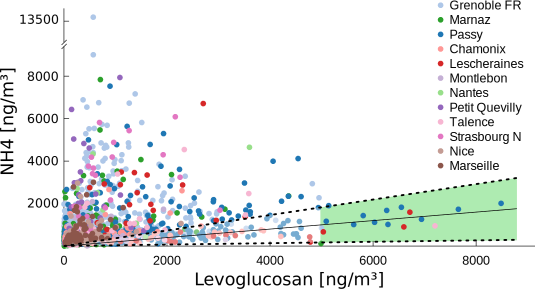
\includegraphics[width=0.7\textwidth]{figures/INACS/MCA_correlNH4Levo_alea.pdf}
    \caption{Estimation du ratio \NHq/lévoglucosan pour les jours de fortes concentrations en
        lévoglucosan. La droite noire en trait plein représente la droite $[\NHq_{bio}]=
        0.221 \times \text{[lévoglucosan]}$, les droites en trait pointillés les
        écart-types considérés ($\frac{1}{8}\times \text{[lévoglucosan]}$) et la zone
        verte les jours où la source de combustion de biomasse est considérée comme
        prépondérante ([lévoglucosan] > \SI{5000}{\ugm}]).
    }
    \label{fig:correlNH4Levo}
\end{figure}


\subsubsection{Principaux résultats}%
\label{ssub:principaux_résultats}

\subsubsection{Conclusion}%
\label{ssub:conclusion}



\subsection{Émission biogénique primaire}%
\label{sub:émission_biogénique_primaire}

\subsection{Processus secondaires}%
\label{sub:processus_secondaires}

\section{SOURCES}%
\label{sec:sources}

\subsection{Introduction}

\subsection{Comparison of PM\textsubscript{10} sources profiles at 15 french sites using a harmonized constrained positive matrix factorization approach}%
\label{sub:article}

\subsection{Conclusion}%
\label{sub:conclusion}



% \includepdf[pages=-,scale=0.9,pagecommand={\pagestyle{fancy}}]{chapters/sources.pdf}

% \subsection{Supporting Information}%
% \label{sub:supporting_information}
%
% \includepdf[pages=-,scale=0.9,pagecommand={\pagestyle{fancy}}]{chapters/SOURCES_SI.pdf}


\section{Conclusion}%
\label{sec:conclusion}

Et aussi LCME: organique (BNT, hopane), EMPA cellulose PM10/PM2.5

Question : SPECIEUROPE et contrainte trop fortes sur certains profils ?

Ouverture : ANDRA et série temporelle

Limitation : 
- espèce trop réactive ? (oxalate ?)
- résolution temporelle



